\documentclass{book}

\usepackage{graphicx}
\usepackage[space]{grffile}
\usepackage{latexsym}
\usepackage{textcomp}
\usepackage{longtable}
\usepackage{multirow,booktabs}
\usepackage{amsfonts,amsmath,amssymb}
\usepackage{natbib}
\usepackage{url}
\usepackage{hyperref}
\hypersetup{colorlinks=false,pdfborder={0 0 0}}
% You can conditionalize code for latexml or normal latex using this.
\newif\iflatexml\latexmlfalse
\usepackage[utf8]{inputenc}
\usepackage[ngerman,english]{babel}

\begin{document}

\author{JP Breuer\\ Affiliation not available  \and Awaiting Activation\\ Affiliation not available \and Awaiting Activation\\ Affiliation not available \and Aaron\\ Affiliation not available \and Yannis\\ Affiliation not available \and FruzsinaBacso\\ Affiliation not available \and Ricard\\ Affiliation not available \and Awaiting Activation\\ Affiliation not available \and Sridhar Remma\\ Affiliation not available \and Gustavo Feijóo\\ Affiliation not available \and Kristian Sloth Lauszus\\ Affiliation not available \and Johannes Linde\\ Affiliation not available \and Maja\\ Affiliation not available \and Agge Winther\\ Affiliation not available \and Paul Connetable\\ Affiliation not available \and Rasmus Lundby Pedersen\\ Affiliation not available}


\title{Spacecraft Instrumentation Europa Life Finder Mission}

\bibliographystyle{plain}

\maketitle

\frontmatter
\tableofcontents
\newpage

\section{Abstract}

NOTE: Default Authoria LATEX class is article. Once finished writing, we change it to book and include Chapters. BOLDED SECTIONS included below are Chapter Titles

\section{Introduction -JP}
% What is our purpose for the mission. Why? How will we achieve our mission objectives? Water, energy, nutrition
% Estimate:
% Mass, Volume, Power budgets
% Why are we going?
    % Are we alone?
    % Water, energy, nutritions
    % Use pasos

Throughout the billions of years of Earth geologic history,it still took several hundreds of millions of years before evolution allowed for complex, intelligent organisms to inhabit the Earth. As soon as free thinking and self-reflection was possible in animals, naturally some of the first questions were the big philosophical ones: What is the origin of life and the universe? What are the conditions necessary to support and develop life? Are we alone in the universe?

Despite advancements in technology,

\section{Problem Formulation}

* Goals

* Focus area - limitations

* Must be answered in the conclusion

* Each subject must add something to the problem formulation

\subsection{Mission Layout and Communication Requirements}

1. Mission Stages from a communications standpoint
    1.1 Journey to Jovian System
    1.2 Descent Maneuver
    1.3 Through-ice communications
    1.4 Science Phase Data Relay
2. General Drivers
3. Assumptions and Models for Europa Communications

\subsection{Problem Limitation}

\section{\textbf{Theory}}


\subsection{Moon Characteristics} % JP, Yannis

* Rock core, water, ice

    * Why do we think so?
    
    * Geysers?
    
\subsubsection{Radiation Environment} % Maja, "landing site guys", "orbiter guys"

* Both for the orbiter and the lander

\subsubsection{Tidal Wave} % Lukas, KSL

\subsection{Ice characteristics} % Lukas, KSL

\subsubsection{Temperature Profile}

* "back of the envelope" calculations

\subsubsection{Pressure Profile}

* What is the outside pressure?

\subsubsection{Structural Profile}

* Ice thickness

* Composition of the ice? % Se: SWRI: "barr-showman-2009" (ask Kristian Lauszus)

* Lakes?

\subsubsection{Simulation Results}

\subsubsection{Simulation Validation}

* Should show that the "back of the envelope" calculations are right

\subsection{What Defines Life?} % Agge, Fruzsi

* Water, oil, fat, carbon, energy

* Proteins (amino acids) etc

* Nutritions, water, heat energy

* How can a life-form be able to convert thermal energy to other forms of energy

* Another energy source could be geysers on the solid core

    * A probe to the ocean bottom might show this
    
* Lakes inside the ice

* Iron-reduction

\subsubsection{Where do we expect to find life?}

* Top or bottom of the water?

* Petri Dish can be used for cultivation

* Steralization of the spacecraft: chemical, heat, radiation

\section{\textbf{Strawman Mission \& Instrument Configuration}} % Akis

See awesome notes by "Johannes Linde"

\subsection{Synthesis}

\section{Orbiter}


\subsection{Orbital Parameters}


\subsection{Design}

\subsubsection{Instruments}

* Teleskope

\subsubsection{Shielding}

\subsubsection{Thermal design}

\subsection{Determination of Landing Site}

\subsubsection{Mapping of the moon}

\subsubsection{Europa Coordinate System}

* How to determine the ice thickness?

* Thinnest ice, smooth area, no boulders, avoid craters

* Radiation

\section{Communication Systems}


\subsection{Earth-to-Orbiter}

1. Introduction and considerations for the link
   1. General Considerations for a Deep Space Mission
   2. HG Link
   3. MG Link
   4. LG Link
   5. Telemetry Uplink/Downlink
   6. Data Downlink
   7. Safe Mode
1. Link Drivers
   1. Dataload
   2. Spacecraft Attitude
1. Link Budget
2. Solution Proposal
3. Drivers to other systems

\subsection{Surface-to-Orbiter}

1. Introduction and considerations for the link
      * (Orbit characteristics and Europa Environment)
1. Link Drivers
   1. Radiation (Europa surf dead zone)
   2. Low Power
   3. Transmission Relay Window
      * Dataload
      * Bitrate
   1. Low Temperature Operation
   2. Line of Sight (viewing angles)
      * Communication while descent maneuver
      * Antenna choice
      * Mechanical stabilizers
1. Link Budget
2. Solution Proposal
3. Drivers to other systems

\subsection{Penetrator-to-Surface}

1. Introduction and considerations for the link
2. Link Drivers
   1. Low Temperature Operation
   2. Low Power
   3. Line of Sight (viewing angles)
      * Vehicle Navigation
      * Antenna choice
   1. Redundancy
   2. Dataload
1. Solution Proposal
   1. Tethered link
      * Solution Layout
         * Specific Drivers
      * Assumptions and Models (Europa Environment)
      * Feasibility assessment
      * Implementation hazards
   1. High directivity link
      * Solution Layout
         * Specific Drivers
      * Assumptions and Models (Europa Environment)
      * Feasibility assessment
      * Implementation hazards
   1. Omnidirectional link
      * Solution Layout
         * Specific Drivers
      * Assumptions and Models (Europa Environment)
      * Feasibility assessment
      * Implementation hazards
   1. Ice embedded Repeaters link
      * Solution Layout
         * Specific Drivers
      * Assumptions and Models (Europa Environment)
      * Feasibility assessment
      * Implementation hazards
    1. Fiber optics
1. Strawman Proposal
   1. Solution Matrix (Score functions)
      * KISS (Keep It Simple Stupid!), Costs, Risks, Flight Ready
   1. Discussion

\subsection{Probe-to-Penetrator}

\section{Lander}

\subsection{Design}

\subsubsection{Thermal design}

\subsection{Navigation}

* IMU, use teleskope on the orbiter

\subsection{Safe landing}

\subsection{Energy source}

* Solar panels

* RTG

* What else?

* We also need heating/cooling

\subsection{Pre-drilling of the hole for the penetrator}


\section{Penetrator}

* What kind of ice can we expect? Mud, silt etc?

\subsection{Drilling Methods}

\subsubsection{Mechanical Drilling}

\subsubsection{Chemical Drilling}

\subsubsection{Explosive Drilling}

\subsubsection{Sputtering}

\subsubsection{Laser Drilling}

\subsubsection{Light Concentration Drilling}

\subsubsection{Melting}

* Water transportation from tip to the end of the penetrator (ref section about convection flow)

* Should measure flow of the water - descent rate

* Water flow to the instruments. Will have to use a pump in order to increase the flow rate.

* Measure conductivity of the water.

\subsection{Selected Design}

* Sketch of overall design (use 3D models for the ice melting simulations)

\subsubsection{Melting through the ice} % Lukas, KSL

\subsubsection{RTG on Top}

\subsubsection{RTG on Bottom}

* How do we protect the rest of the instruments against the radiation?

\subsubsection{RTG design}

* Can we make it smaller?

* Thermal design

\subsubsection{Thermal Design}

\subsubsection{Water Convection}

\subsubsection{Anchor Design}

\subsubsection{Anchoring and Deployment}

* Ref to composition of the ice and theory about lakes?

\subsubsection{Submarine}

\subsection{Mechanisms and Instrumentation}

\subsubsection{Navigation and Dirigibility}

\subsubsection{Detection of Depth and End of Ice Column}

* Echo sounder etc

\subsection{Communication Systems}


\subsubsection{Ice Losses}
As we expect, Europa's subsurface consists mainly of several kilometers of ice, which we want to penetrate with electromagnetic waves to establish the communication link between the penetrator and the lander vehicle. Fortunately, a lot of research has been made in the recent decades on how efficient an electromagnetic wave can penetrate different ice layers and on which parameters can affect this propagation. These principles are applied widely in subsurface radar sounding that take place in polar areas, but also in planetary exploration (Mars). For a wide range of frequencies, ranging from MHz to GHz, dielectric losses of ice are independent of frequency. By that it is meant that, the number of wavelengths, which can penetrate into ice before being attenuated to a given fraction of its initial amplitude ($1/e$ of initial amplitude) is approximately the same regardless of frequency. The above implies that the longer the wavelength, the deeper the radar signal can penetrate before being attenuated below the detection of our equipment. Thus, deep ice penetration requires that the radar operates at the lowest possible frequency. 

\paragraph{Dielectric properties of ice}
(For the following two paragraphs \cite{Kofman_2010} has used as main reference.)The permittivity $\epsilon$ of a material is a property describing how much more energy is stored though change separation than in vacuum. Frequency dependence of permittivity occurs because change separation does not happen instantaneously. Changes separate with finite velocities, thus if the external field is reversing polarity too quickly the changes cannot move fast enough to keep up. The frequency at which the charges fully separate and are in constant motion is called the relaxation frequency. At frequencies below the relaxation frequency the permittivity plateaus at the low frequency limit (static) $\epsilon_{s}$, which is often call dielectric constant. At high frequencies above the relaxation frequency the permittivity plateaus at the high frequency limit $\epsilon_{\infty}$. Moreover, ice crystal formation has an impact on polarization, which primarily depends on temperature.

Debye model takes into account the above mentioned theory about dielectric constant of ice and is described by the following equations: 

\begin{equation}
    \epsilon=\epsilon_{\infty}+\Delta \epsilon \frac{\Delta \epsilon}{1+j \omega \tau}
    \label{dielectric}
\end{equation}

, where $\omega = 2\pi f$, $\Delta \epsilon=\epsilon_{s} -\epsilon_{\infty}$ and $\tau$ is the dielectric relaxation time. \\
The permittivity is a complex function of frequency and usually is described by its real and imaginary part.

\begin{equation}
    Re (\epsilon)=\epsilon_{\infty}+\Delta \epsilon \frac{\Delta \epsilon}{1+ \omega^2 \tau^2}
    \label{real}
\end{equation}

\begin{equation}
    Im (\epsilon)=\frac{\Delta \epsilon\ \omega\  \tau}{1+ \omega^2 \tau^2}
    \label{imag}
\end{equation}
The loss tangent (tan $\delta$) is defined by the ratio of these two parts and characterizes the attenuation of the electromagnetic waves in a medium due to ohmic conductivity $\sigma$. 

\begin{equation}
    tan \delta=\frac{Re(\epsilon)}{Im(\epsilon)}=\frac{\sigma}{\omega\ Re(\epsilon)}
    \label{tan}
\end{equation}
The conductivity $\sigma$ of the medium is directly proportional to the imaginary part of the dielectric constant.

Because of the complexity of equations (\ref{dielectric} - \ref{tan}) an approximated expression has been developed to compute the attenuation.

\begin{multline}
    a=0.129 \sqrt{Re(\epsilon)}\ f (\sqrt{1+tan^2 \delta}-1)^{1/2} \approx \\
    \approx 0.091 \sqrt{Re(\epsilon)}\ f\ tan \delta \approx 0.0009\ \sigma\ dB/m
    \label{losses}
\end{multline}
where, $\sigma$ is in $\mu S m^{-1}$. As one can see from eq. (\ref{losses}), attenuation's value is directly proportional to frequency, or in other words to the conductivity of the medium. Additionally, the static dielectric constant of pure ice is heavily depended on the orientation of electric field with respect to the crystal's axis. The effect of pressure is about 1\% per kbar for polycrystalline ice \cite{Kofman_2010}. The above formulas and their approximations concerning the electromagnetic waves can be used adequately for very low temperatures, as the ranges we are interested.

Nevertheless, the losses due to pure ice are well documented in bibliography, there is a big gap regarding ice impurities on icy moons. The absence of these data are due to uncertainties and lack of knowledge of the physical nature of impurities on these satellites. This problem was studied by  Moore \cite{Moore_2000} and Chyba \cite{Chyba_1998} for Europa. Moore considered three types of water ice on Europa, produced by three basic processes occurring on Earth. The first one is meteoric ice formed by atmospheric precipitations, sea ice formed by the freezing of water close to the atmospheric interface and marine ice forming beneath ice shelves directly from ocean water. Moore concluded that similar processes are likely to occur on Europa as well, and that the most probable form of ice would be marine ice. In figure \ref{impurities} Moore sums up the attenuation from different type of impurities in ice \cite{Moore_2000}.

\begin{figure}[ht]
\centering
\label{impurities}
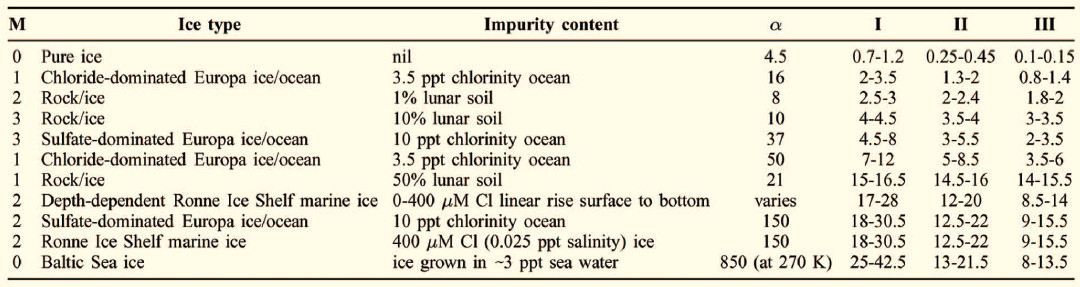
\includegraphics[width=1\textwidth]{figures/Moore2.jpg}
\caption{Attenuation, $a$, is in dB/km at 251 K and corresponds to the one way attenuation due to  ice impurities, in case of a sounding radar. Columns I, II, and III are computed one-way attenuation, in dB/km, for ice shells with base temperatures of 270, 260, and 250 K, respectively. The range of values for each of these corresponds to surface temperatures of 50 and 100 K. These values are independent of shell thickness since the temperature profile is stretched to the ice thickness. The M column represents the plausibility of the ice type for Europa; 0 is least likely while 3 is more likely, given the present understanding
of Europa. The distribution coefficients $k_{0}$ and $k_{MI}$ affecting the marine ice models come from laboratory experiments \cite{Moore_2000}. \textbf{+ appendix}}
\end{figure}
The above calculations data are not taking into account a possible scattering mechanism of electromagnetic wave due to ice layers that can exist in the crust. The scattering effect has a significant impact on the attenuation level and depends strongly on the dimensions of cavities in the medium compared to the wavelength. The two main mechanisms of scattering coming from the ice crust are surface scattering and scattering by volume irregularities. Both these effects can change considerably the penetration depth of the wave into the ice, but also the ratio of any subsurface echo to surface clutter. As we can understand the scattering depends strongly on the wavelength and surface parameters of the body under investigation. 

The conclusion is that the expected one way attenuation because of impurities of ice is in the range 1-8 dB/Km and this number is independent of the frequency. Although, the frequency dependence of attenuation due to scattering mechanisms dictates the use of as low frequencies as possible in order to achieve a deep penetration. The main bottlenecks in that case are two. The first one is that the choice of frequency has an influence on the characteristics of instrumentation and especially on the size of the antenna and the second one is Jupiter's radio emissions spectrum. Figure \ref{J_spec} depicts how Jupiter's activity affect the electromagnetic environment of its moons. Clearly can be seen that frequencies from almost zero Hz up to 50 MHz are dominated from Jupiter's radio emissions. Thus, the exact choice of frequency results in a trade off between science requirements and technical limitations taking into account also the physical constraints of the environment under research. 

\begin{figure}[ht]
\centering
\label{J_spec}
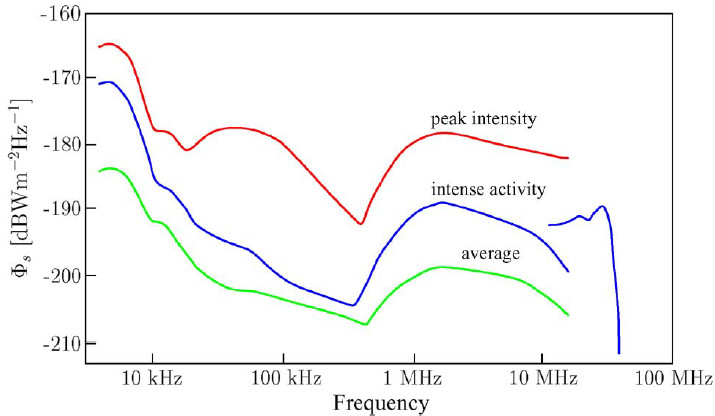
\includegraphics[width=0.7\textwidth]{figures/below100.jpg}
\caption{Jupiter radio spectrum based on Cassini-RPWS data,
normalized to a distance of 1 AU. Green curve: rotation averaged
emission. Blue curve: rotation averaged emission at times of intense
activity. Red curve: peak intensities during active periods. \cite{Grie_meier_2005}}
\end{figure}


\begin{figure}[ht]
\begin{center}
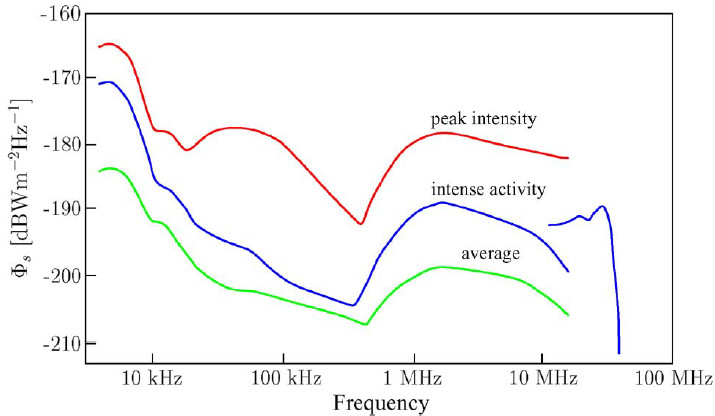
\includegraphics[width=0.7\columnwidth]{figures/below100}
\caption{Replace this text with your caption%
}
\end{center}
\end{figure}

\subsubsection{Communication to Lander}


\subsubsection{High Directivity Link}

\subsubsection{Relay Systems}


\section{Instrument Suite}

* Total mass and power requirement

* What do we want to measure and why? Explain why some instruments were picked and some were discarded (we can use the notes from when we did that in class)

\subsection{Up-concentration}

\subsection{Water flow for the instruments} % Figure out a better title?

* Water convection is not enough. We need a pump (peristaltic pump).

\subsection{Sample handling}

* We need a design, I (Kristian) talked with some other about this, but we need to coordinate with the rest of the groups

* Sample rate

* What is under pressure and what is not?

* Order of the instruments


\subsection{CTD/ADCP} % Sridhar

* Includes temperature probe

    * We will properly need more around the body of the penetrator

\subsection{Light sensor}

\subsection{Gas detection}

\subsection{XRF}

\subsection{Lab-in-a-Chip Systems}


\subsection{pH \& salinity}

\subsection{Camera}

\subsection{Microscope}

\section{Analysis, Verification, and Viability}

* Redundancy

\section{Conclusion}

* Tied to Problem Formulation

\section{Future Work}

* Hard to test due to time limits, limited funds etc

    * Instruments are expensive and might be hard to get (fx RTG)

\bibliography{bibliography/biblio.bib%
}

\end{document}

